% ═══════════════════════════════════════════════════════════════════════════════
\section{Analýza personalizácie: Porovnanie dvoch používateľov}
% ═══════════════════════════════════════════════════════════════════════════════

V tejto časti porovnávame správanie odporúčacieho algoritmu pre dvoch používateľov s odlišnou históriou návštev a záujmami. Obaja dostali identické nastavenia váh v každom testovacom scenári, čo umožňuje priamo pozorovať, ako história a obľúbené eventy ovplyvňujú výsledky odporúčania.

% ───────────────────────────────────────────────────────────────────────────────
\subsection{Profil používateľa Test User 31}
% ───────────────────────────────────────────────────────────────────────────────

Používateľ Test User 31 navštívil celkovo 10 udalostí z rôznych kategórií, čo naznačuje širokospektrálny záujem bez dominantnej témy. Rozdelenie podľa hlavných kategórií je spracované v tabuľke \ref{tab:rozdelenie_u31}.

\begin{table}[H]
\centering
\caption{Rozdelenie návštev podľa kategórií – Test User 31}
\label{tab:rozdelenie_u31}
\begin{tabular}{|l|c|}
\hline
\textbf{Kategória} & \textbf{Počet návštev} \\ \hline
Music \& Entertainment & 4 \\
Sports                 & 2 \\
Nature \& Outdoor      & 1 \\
Art \& Culture         & 1 \\
Community \& Social    & 1 \\
Business \& Tech       & 1 \\ \hline
\textbf{Spolu}         & \textbf{10} \\ \hline
\end{tabular}
\end{table}

\begin{table}[H]
\centering
\caption{Konkrétne navštívené udalosti – Test User 31}
\label{tab:eventy_u31}
\small
\begin{tabular}{|l|l|l|}
\hline
\textbf{Názov udalosti} & \textbf{Podkategória} & \textbf{Kategória} \\ \hline
udalost 7 \#171  & Watercraft sports         & Sports \\
udalost 3 \#92   & Speed dating              & Community \& Social \\
udalost 8 \#7    & Iný koncert               & Music \& Entertainment \\
udalost 15 \#14  & DJ Set                    & Music \& Entertainment \\
udalost 1 \#105  & Výstava                   & Art \& Culture \\
udalost 5 \#154  & Karaoke                   & Music \& Entertainment \\
udalost 7 \#66   & Botanická záhrada         & Nature \& Outdoor \\
udalost 10 \#129 & Individual sports         & Sports \\
udalost 12 \#116 & DJ Set                    & Music \& Entertainment \\
udalost 9 \#173  & Pitch Night               & Business \& Tech \\ \hline
\end{tabular}
\end{table}

Okrem histórie návštev označil používateľ 4 udalosti ako obľúbené, pričom všetky pochádzajú z kategórie \textit{Music \& Entertainment}, čo posilňuje jeho implicitný záujem o túto kategóriu (tabuľka \ref{tab:oblubene_u31}).

\begin{table}[H]
\centering
\caption{Obľúbené udalosti – Test User 31}
\label{tab:oblubene_u31}
\begin{tabular}{|l|l|l|}
\hline
\textbf{Názov udalosti} & \textbf{Podkategória} & \textbf{Kategória} \\ \hline
udalost 5 \#154  & Karaoke           & Music \& Entertainment \\
udalost 7 \#66   & Botanická záhrada & Nature \& Outdoor \\
udalost 15 \#14  & DJ Set            & Music \& Entertainment \\
udalost 8 \#7    & Iný koncert       & Music \& Entertainment \\ \hline
\end{tabular}
\end{table}

\begin{figure}[H]
\centering
\begin{minipage}{0.48\textwidth}
    \centering
    \begin{tikzpicture}[scale=0.7]
        \tikzset{every node/.style={font=\scriptsize}}
        \pie[text=legend, radius=1.8,
             color={blue!60, green!60, orange!60, red!60, cyan!60, violet!60}]{
            40/Music \& Ent.,
            20/Sports,
            10/Nature,
            10/Art \& Culture,
            10/Community,
            10/Business
        }
    \end{tikzpicture}
    \caption{Hlavné kategórie}
\end{minipage}
\hfill
\begin{minipage}{0.48\textwidth}
    \centering
    \begin{tikzpicture}[scale=0.7]
        \tikzset{every node/.style={font=\scriptsize}}
        \pie[text=legend, radius=1.8,
             color={blue!60, cyan!60, green!60, orange!60, red!60, gray!60, violet!60}]{
            20/DJ Set,
            10/Iný koncert,
            10/Karaoke,
            10/Watercraft,
            10/Individual,
            10/Speed dating,
            30/Ostatné
        }
    \end{tikzpicture}
    \caption{Podkategórie}
\end{minipage}
\caption{Preferencie Test User 31 – kategórie a podkategórie}
\label{fig:profil_u31}
\end{figure}

% ───────────────────────────────────────────────────────────────────────────────
\subsection{Profil používateľa Test User 19}
% ───────────────────────────────────────────────────────────────────────────────

Používateľ Test User 19 navštívil 5 udalostí a vykazuje výraznejšiu koncentráciu záujmov – prevažujú \textit{Sports} a \textit{Education}. Má iba jednu obľúbenú udalosť, čo obmedzuje vplyv faktora $B_{fav}$ na odporúčania.

\begin{table}[H]
\centering
\caption{Rozdelenie návštev podľa kategórií – Test User 19}
\label{tab:rozdelenie_u19}
\begin{tabular}{|l|c|}
\hline
\textbf{Kategória} & \textbf{Počet návštev} \\ \hline
Sports              & 2 \\
Education           & 2 \\
Community \& Social & 1 \\ \hline
\textbf{Spolu}      & \textbf{5} \\ \hline
\end{tabular}
\end{table}

\begin{table}[H]
\centering
\caption{Konkrétne navštívené udalosti – Test User 19}
\label{tab:eventy_u19}
\small
\begin{tabular}{|l|l|l|}
\hline
\textbf{Názov udalosti} & \textbf{Podkategória} & \textbf{Kategória} \\ \hline
udalost 7 \#171 & Watercraft sports        & Sports \\
udalost 9 \#38  & E-sports (comp. gaming)  & Sports \\
udalost 1 \#120 & Osobný rozvoj            & Education \\
udalost 3 \#2   & Street meetup            & Community \& Social \\
udalost 10 \#39 & Jazykový kurz            & Education \\ \hline
\end{tabular}
\end{table}

\begin{table}[H]
\centering
\caption{Obľúbené udalosti – Test User 19}
\label{tab:oblubene_u19}
\begin{tabular}{|l|l|l|}
\hline
\textbf{Názov udalosti} & \textbf{Podkategória} & \textbf{Kategória} \\ \hline
udalost 3 \#2 & Street meetup & Community \& Social \\ \hline
\end{tabular}
\end{table}

\begin{figure}[H]
\centering
\begin{minipage}{0.48\textwidth}
    \centering
    \begin{tikzpicture}[scale=0.7]
        \tikzset{every node/.style={font=\scriptsize}}
        \pie[text=legend, radius=1.8,
             color={blue!60, green!60, orange!60}]{
            40/Sports,
            40/Education,
            20/Community
        }
    \end{tikzpicture}
    \caption{Hlavné kategórie}
\end{minipage}
\hfill
\begin{minipage}{0.48\textwidth}
    \centering
    \begin{tikzpicture}[scale=0.7]
        \tikzset{every node/.style={font=\scriptsize}}
        \pie[text=legend, radius=1.8,
             color={blue!60, cyan!60, green!60, orange!60, red!60}]{
            20/Watercraft,
            20/E-sports,
            20/Osobný rozvoj,
            20/Street meetup,
            20/Jazykový kurz
        }
    \end{tikzpicture}
    \caption{Podkategórie}
\end{minipage}
\caption{Preferencie Test User 19 – kategórie a podkategórie}
\label{fig:profil_u19}
\end{figure}

% ═══════════════════════════════════════════════════════════════════════════════
\subsection{Porovnávacie testovanie}
% ═══════════════════════════════════════════════════════════════════════════════

V nasledujúcich scenároch dostali obaja používatelia identické nastavenie váh. Každý test obsahuje konfiguráciu váh, výsledok TOP~1 odporúčania pre každého používateľa a spoločný vizuálny rozbor príspevkov faktorov k výslednému skóre.

% ───────────────────────────────────────────────────────────────────────────────
\subsubsection{Test A: Dominancia obľúbeného bonusu ($w_6 = 60\,\%$)}
% ───────────────────────────────────────────────────────────────────────────────

\begin{table}[H]
\centering
\caption{Konfigurácia váh – Test A}
\label{tab:vahy_testA}
\begin{tabular}{|l|c|}
\hline
\textbf{Faktor} & \textbf{Váha ($w_i$)} \\ \hline
Hlavná kategória ($w_1$) & 8\% \\
Podkategória ($w_2$)     & 8\% \\
Vzdialenosť ($w_3$)      & 8\% \\
Rating ($w_4$)           & 8\% \\
Popularita ($w_5$)       & 8\% \\
Obľúbený bonus ($w_6$)   & 60\% \\ \hline
\textbf{Súčet}           & \textbf{100\%} \\ \hline
\end{tabular}
\end{table}

\begin{table}[H]
\centering
\caption{TOP 1 odporúčanie – Test A}
\label{tab:vysledky_testA}
\small
\begin{tabular}{|l|l|l|}
\hline
 & \textbf{Test User 31} & \textbf{Test User 19} \\ \hline
\textbf{Udalosť}      & udalost 14 \#163          & udalost 10 \#99 \\
\textbf{Kategória}    & Music \& Ent. / Iný koncert & Community \& Social / Street meetup \\
\textbf{Vzdialenosť}  & 5.49 km                   & 8.63 km \\
\textbf{Rating}       & 4.8 / 5 (3 hod.)          & 4.1 / 5 (12 hod.) \\
\textbf{Účastníci}    & 8/17                      & 6/30 \\ \hline
\textbf{Celkové skóre} & \textbf{80.6\%}          & \textbf{75.7\%} \\ \hline
Hl. kategória         & 3.2\%                     & 1.6\% \\
Podkategória          & 0.8\%                     & 1.6\% \\
Vzdialenosť           & 5.2\%                     & 4.3\% \\
Rating                & 7.7\%                     & 6.6\% \\
Popularita            & 3.8\%                     & 1.6\% \\
Obľúbený bonus        & 60.0\%                    & 60.0\% \\ \hline
\end{tabular}
\end{table}

\begin{figure}[H]
\centering
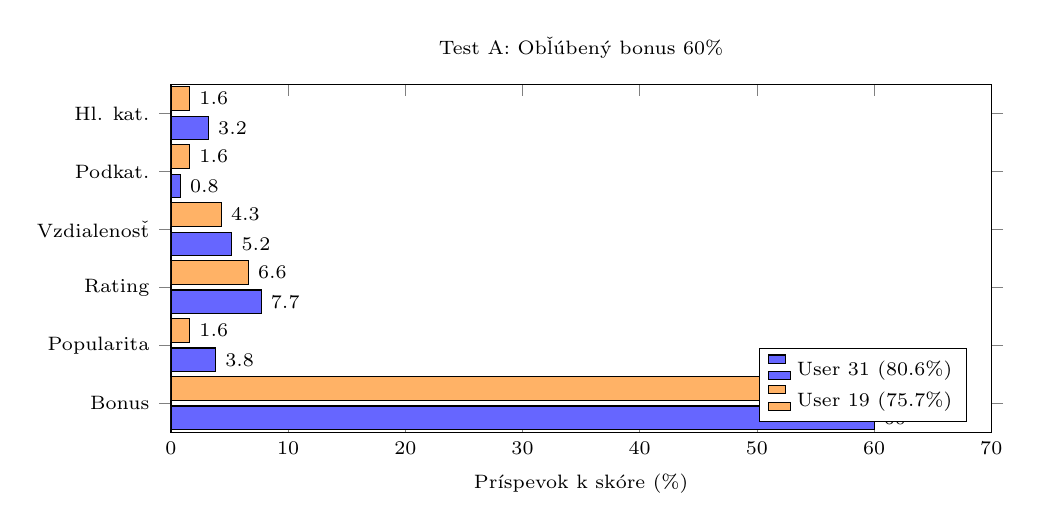
\begin{tikzpicture}
\begin{axis}[
    xbar, width=12cm, height=6cm,
    xlabel={Príspevok k skóre (\%)},
    symbolic y coords={Bonus, Popularita, Rating, Vzdialenosť, Podkat., Hl. kat.},
    ytick=data,
    nodes near coords,
    nodes near coords align={horizontal},
    title={Test A: Obľúbený bonus 60\%},
    xmin=0, xmax=70,
    bar width=0.3cm,
    legend style={at={(1.0,0.3)}, anchor=east},
    legend pos=south east,
]
\addplot[fill=blue!60] coordinates {
    (3.2,Hl. kat.) (0.8,Podkat.) (5.2,Vzdialenosť) (7.7,Rating) (3.8,Popularita) (60.0,Bonus)
};
\addplot[fill=orange!60] coordinates {
    (1.6,Hl. kat.) (1.6,Podkat.) (4.3,Vzdialenosť) (6.6,Rating) (1.6,Popularita) (60.0,Bonus)
};
\legend{User 31 (80.6\%), User 19 (75.7\%)}
\end{axis}
\end{tikzpicture}
\caption{Porovnanie príspevkov faktorov – Test A}
\label{fig:graf_testA}
\end{figure}

Pri dominancii obľúbeného bonusu obaja používatelia dostali odporúčanie z kategórie zhodnej s ich obľúbenými udalosťami. User 31 (4 obľúbené z Music \& Entertainment) dosiahol vyššie celkové skóre 80.6\,\% oproti User 19 (1 obľúbená), keďže viac obľúbených eventov zvyšuje pravdepodobnosť zhody s ďalšími podujatiami od rovnakých organizátorov alebo kategórií.

% ───────────────────────────────────────────────────────────────────────────────
\subsubsection{Test B: Dominancia popularity ($w_5 = 60\,\%$)}
% ───────────────────────────────────────────────────────────────────────────────

\begin{table}[H]
\centering
\caption{Konfigurácia váh – Test B}
\label{tab:vahy_testB}
\begin{tabular}{|l|c|}
\hline
\textbf{Faktor} & \textbf{Váha ($w_i$)} \\ \hline
Hlavná kategória ($w_1$) & 8\% \\
Podkategória ($w_2$)     & 8\% \\
Vzdialenosť ($w_3$)      & 8\% \\
Rating ($w_4$)           & 8\% \\
Popularita ($w_5$)       & 60\% \\
Obľúbený bonus ($w_6$)   & 8\% \\ \hline
\textbf{Súčet}           & \textbf{100\%} \\ \hline
\end{tabular}
\end{table}

\begin{table}[H]
\centering
\caption{TOP 1 odporúčanie – Test B}
\label{tab:vysledky_testB}
\small
\begin{tabular}{|l|l|l|}
\hline
 & \textbf{Test User 31} & \textbf{Test User 19} \\ \hline
\textbf{Udalosť}      & udalost 2 \#46              & udalost 2 \#46 \\
\textbf{Kategória}    & Art \& Culture / Maľovanie  & Art \& Culture / Maľovanie \\
\textbf{Vzdialenosť}  & 9.93 km                     & 6.87 km \\
\textbf{Rating}       & 4.2 / 5 (11 hod.)           & 4.2 / 5 (11 hod.) \\
\textbf{Účastníci}    & 7/8                         & 7/8 \\ \hline
\textbf{Celkové skóre} & \textbf{64.0\%}            & \textbf{64.3\%} \\ \hline
Hl. kategória         & 0.8\%                       & 0.4\% \\
Podkategória          & 0.0\%                       & 0.0\% \\
Vzdialenosť           & 4.0\%                       & 4.7\% \\
Rating                & 6.7\%                       & 6.7\% \\
Popularita            & 52.5\%                      & 52.5\% \\
Obľúbený bonus        & 0.0\%                       & 0.0\% \\ \hline
\end{tabular}
\end{table}

\begin{figure}[H]
\centering
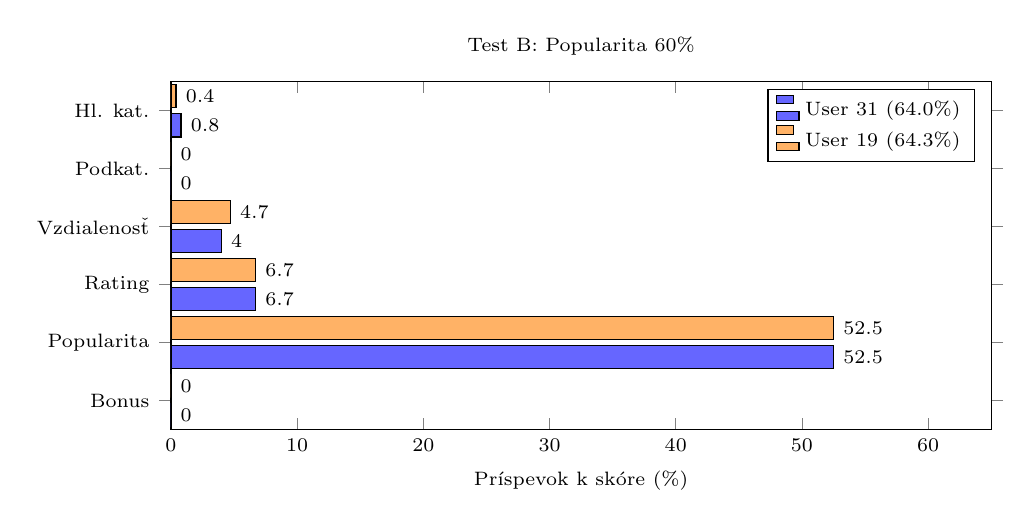
\begin{tikzpicture}
\begin{axis}[
    xbar, width=12cm, height=6cm,
    xlabel={Príspevok k skóre (\%)},
    symbolic y coords={Bonus, Popularita, Rating, Vzdialenosť, Podkat., Hl. kat.},
    ytick=data,
    nodes near coords,
    nodes near coords align={horizontal},
    title={Test B: Popularita 60\%},
    xmin=0, xmax=65,
    bar width=0.3cm,
]
\addplot[fill=blue!60] coordinates {
    (0.8,Hl. kat.) (0.0,Podkat.) (4.0,Vzdialenosť) (6.7,Rating) (52.5,Popularita) (0.0,Bonus)
};
\addplot[fill=orange!60] coordinates {
    (0.4,Hl. kat.) (0.0,Podkat.) (4.7,Vzdialenosť) (6.7,Rating) (52.5,Popularita) (0.0,Bonus)
};
\legend{User 31 (64.0\%), User 19 (64.3\%)}
\end{axis}
\end{tikzpicture}
\caption{Porovnanie príspevkov faktorov – Test B}
\label{fig:graf_testB}
\end{figure}

Tento test odhaľuje kľúčový jav: \textbf{obaja používatelia dostali identické odporúčanie} (udalost 2 \#46 – Art \& Culture / Maľovanie), napriek tomu, že ani jeden z nich túto kategóriu v histórii nenavštívil. Skóre sa líši minimálne (64.0\,\% vs 64.3\,\%) – rozdiel spôsobila mierne odlišná vzdialenosť k tejto udalosti. Popularita ako dominantný faktor potláča personalizáciu a favorizuje udalosti s vysokou obsadenosťou kapacity bez ohľadu na záujmy používateľa.

% ───────────────────────────────────────────────────────────────────────────────
\subsubsection{Test C: Dominancia vzdialenosti ($w_3 = 60\,\%$)}
% ───────────────────────────────────────────────────────────────────────────────

\begin{table}[H]
\centering
\caption{Konfigurácia váh – Test C}
\label{tab:vahy_testC}
\begin{tabular}{|l|c|}
\hline
\textbf{Faktor} & \textbf{Váha ($w_i$)} \\ \hline
Hlavná kategória ($w_1$) & 8\% \\
Podkategória ($w_2$)     & 8\% \\
Vzdialenosť ($w_3$)      & 60\% \\
Rating ($w_4$)           & 8\% \\
Popularita ($w_5$)       & 8\% \\
Obľúbený bonus ($w_6$)   & 8\% \\ \hline
\textbf{Súčet}           & \textbf{100\%} \\ \hline
\end{tabular}
\end{table}

\begin{table}[H]
\centering
\caption{TOP 1 odporúčanie – Test C}
\label{tab:vysledky_testC}
\small
\begin{tabular}{|l|l|l|}
\hline
 & \textbf{Test User 31} & \textbf{Test User 19} \\ \hline
\textbf{Udalosť}      & udalost 9 \#68                    & udalost 5 \#169 \\
\textbf{Kategória}    & Nature \& Outdoor / Bot. záhrada  & Sports / Individual sports \\
\textbf{Vzdialenosť}  & 1.84 km                           & 0.27 km \\
\textbf{Rating}       & 3.6 / 5 (16 hod.)                 & 3.3 / 5 (15 hod.) \\
\textbf{Účastníci}    & 4/29                              & 8/26 \\ \hline
\textbf{Celkové skóre} & \textbf{67.2\%}                  & \textbf{69.3\%} \\ \hline
Hl. kategória         & 0.8\%                             & 3.2\% \\
Podkategória          & 0.8\%                             & 0.0\% \\
Vzdialenosť           & 50.7\%                            & 58.4\% \\
Rating                & 5.8\%                             & 5.2\% \\
Popularita            & 1.1\%                             & 2.5\% \\
Obľúbený bonus        & 8.0\%                             & 0.0\% \\ \hline
\end{tabular}
\end{table}

\begin{figure}[H]
\centering
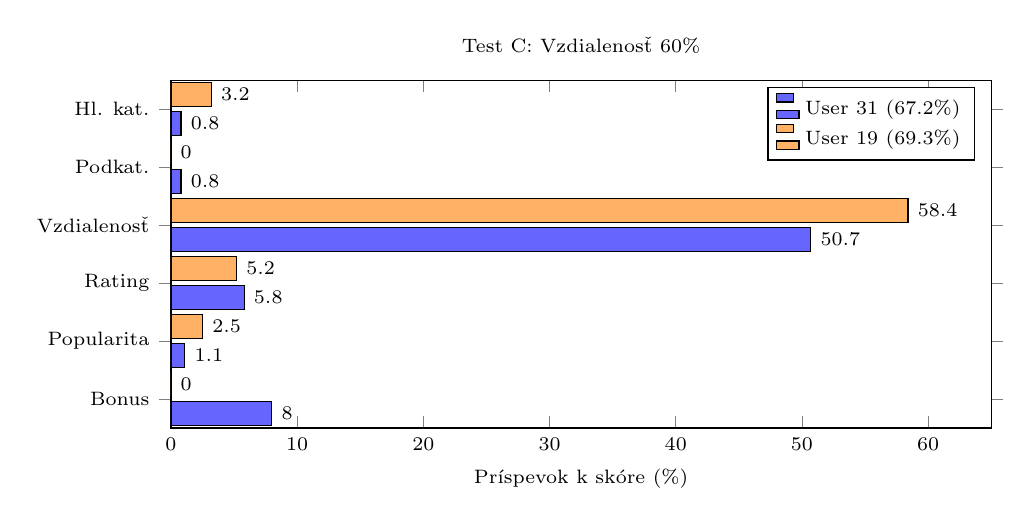
\begin{tikzpicture}
\begin{axis}[
    xbar, width=12cm, height=6cm,
    xlabel={Príspevok k skóre (\%)},
    symbolic y coords={Bonus, Popularita, Rating, Vzdialenosť, Podkat., Hl. kat.},
    ytick=data,
    nodes near coords,
    nodes near coords align={horizontal},
    title={Test C: Vzdialenosť 60\%},
    xmin=0, xmax=65,
    bar width=0.3cm,
]
\addplot[fill=blue!60] coordinates {
    (0.8,Hl. kat.) (0.8,Podkat.) (50.7,Vzdialenosť) (5.8,Rating) (1.1,Popularita) (8.0,Bonus)
};
\addplot[fill=orange!60] coordinates {
    (3.2,Hl. kat.) (0.0,Podkat.) (58.4,Vzdialenosť) (5.2,Rating) (2.5,Popularita) (0.0,Bonus)
};
\legend{User 31 (67.2\%), User 19 (69.3\%)}
\end{axis}
\end{tikzpicture}
\caption{Porovnanie príspevkov faktorov – Test C}
\label{fig:graf_testC}
\end{figure}

Pri maximalizácii váhy vzdialenosti systém uprednostnil geograficky najbližšie podujatia bez ohľadu na tematickú zhodu. User 19 dosiahol vyššie skóre (69.3\,\%) vďaka udalosti vzdialenej iba 0.27\,km, ktorá tak dominuje výsledku napriek priemernému ratingu 3.3.

% ───────────────────────────────────────────────────────────────────────────────
\subsubsection{Test D: Dominancia ratingu ($w_4 = 60\,\%$)}
% ───────────────────────────────────────────────────────────────────────────────

\begin{table}[H]
\centering
\caption{Konfigurácia váh – Test D}
\label{tab:vahy_testD}
\begin{tabular}{|l|c|}
\hline
\textbf{Faktor} & \textbf{Váha ($w_i$)} \\ \hline
Hlavná kategória ($w_1$) & 8\% \\
Podkategória ($w_2$)     & 8\% \\
Vzdialenosť ($w_3$)      & 8\% \\
Rating ($w_4$)           & 60\% \\
Popularita ($w_5$)       & 8\% \\
Obľúbený bonus ($w_6$)   & 8\% \\ \hline
\textbf{Súčet}           & \textbf{100\%} \\ \hline
\end{tabular}
\end{table}

\begin{table}[H]
\centering
\caption{TOP 1 odporúčanie – Test D}
\label{tab:vysledky_testD}
\small
\begin{tabular}{|l|l|l|}
\hline
 & \textbf{Test User 31} & \textbf{Test User 19} \\ \hline
\textbf{Udalosť}      & udalost 14 \#163            & udalost 12 \#26 \\
\textbf{Kategória}    & Music \& Ent. / Iný koncert & Community \& Social / Street meetup \\
\textbf{Vzdialenosť}  & 5.49 km                     & 21.70 km \\
\textbf{Rating}       & 4.8 / 5 (3 hod.)            & 5.0 / 5 (13 hod.) \\
\textbf{Účastníci}    & 8/17                        & 6/34 \\ \hline
\textbf{Celkové skóre} & \textbf{78.7\%}            & \textbf{74.9\%} \\ \hline
Hl. kategória         & 3.2\%                       & 1.6\% \\
Podkategória          & 0.8\%                       & 1.6\% \\
Vzdialenosť           & 5.2\%                       & 2.5\% \\
Rating                & 57.8\%                      & 59.7\% \\
Popularita            & 3.8\%                       & 1.4\% \\
Obľúbený bonus        & 8.0\%                       & 8.0\% \\ \hline
\end{tabular}
\end{table}

\begin{figure}[H]
\centering
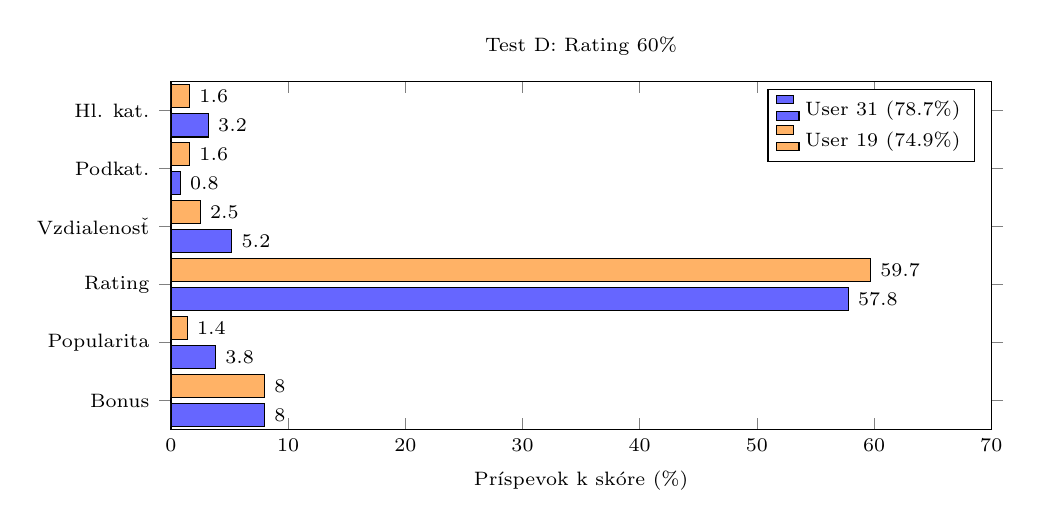
\begin{tikzpicture}
\begin{axis}[
    xbar, width=12cm, height=6cm,
    xlabel={Príspevok k skóre (\%)},
    symbolic y coords={Bonus, Popularita, Rating, Vzdialenosť, Podkat., Hl. kat.},
    ytick=data,
    nodes near coords,
    nodes near coords align={horizontal},
    title={Test D: Rating 60\%},
    xmin=0, xmax=70,
    bar width=0.3cm,
]
\addplot[fill=blue!60] coordinates {
    (3.2,Hl. kat.) (0.8,Podkat.) (5.2,Vzdialenosť) (57.8,Rating) (3.8,Popularita) (8.0,Bonus)
};
\addplot[fill=orange!60] coordinates {
    (1.6,Hl. kat.) (1.6,Podkat.) (2.5,Vzdialenosť) (59.7,Rating) (1.4,Popularita) (8.0,Bonus)
};
\legend{User 31 (78.7\%), User 19 (74.9\%)}
\end{axis}
\end{tikzpicture}
\caption{Porovnanie príspevkov faktorov – Test D}
\label{fig:graf_testD}
\end{figure}

Pri dominancii ratingu systém uprednostnil najlepšie hodnotené podujatia. Zaujímavý kontrast predstavuje User 19, ktorému bolo odporúčané podujatie vzdialené 21.70\,km (najvzdialenejší výsledok spomedzi všetkých testov) – rating 5.0 plne prekryl geografický handicap.

% ───────────────────────────────────────────────────────────────────────────────
\subsubsection{Test E: Dominancia hlavnej kategórie ($w_1 = 60\,\%$)}
% ───────────────────────────────────────────────────────────────────────────────

\begin{table}[H]
\centering
\caption{Konfigurácia váh – Test E}
\label{tab:vahy_testE}
\begin{tabular}{|l|c|}
\hline
\textbf{Faktor} & \textbf{Váha ($w_i$)} \\ \hline
Hlavná kategória ($w_1$) & 60\% \\
Podkategória ($w_2$)     & 8\% \\
Vzdialenosť ($w_3$)      & 8\% \\
Rating ($w_4$)           & 8\% \\
Popularita ($w_5$)       & 8\% \\
Obľúbený bonus ($w_6$)   & 8\% \\ \hline
\textbf{Súčet}           & \textbf{100\%} \\ \hline
\end{tabular}
\end{table}

\begin{table}[H]
\centering
\caption{TOP 1 odporúčanie – Test E}
\label{tab:vysledky_testE}
\small
\begin{tabular}{|l|l|l|}
\hline
 & \textbf{Test User 31} & \textbf{Test User 19} \\ \hline
\textbf{Udalosť}      & udalost 14 \#163            & udalost 11 \#190 \\
\textbf{Kategória}    & Music \& Ent. / Iný koncert & Sports / Extreme sports \\
\textbf{Vzdialenosť}  & 5.49 km                     & 1.76 km \\
\textbf{Rating}       & 4.8 / 5 (3 hod.)            & 4.6 / 5 (11 hod.) \\
\textbf{Účastníci}    & 8/17                        & 6/13 \\ \hline
\textbf{Celkové skóre} & \textbf{49.4\%}            & \textbf{41.9\%} \\ \hline
Hl. kategória         & 24.0\%                      & 24.0\% \\
Podkategória          & 0.8\%                       & 0.0\% \\
Vzdialenosť           & 5.2\%                       & 6.8\% \\
Rating                & 7.7\%                       & 7.4\% \\
Popularita            & 3.8\%                       & 3.7\% \\
Obľúbený bonus        & 8.0\%                       & 0.0\% \\ \hline
\end{tabular}
\end{table}

\begin{figure}[H]
\centering
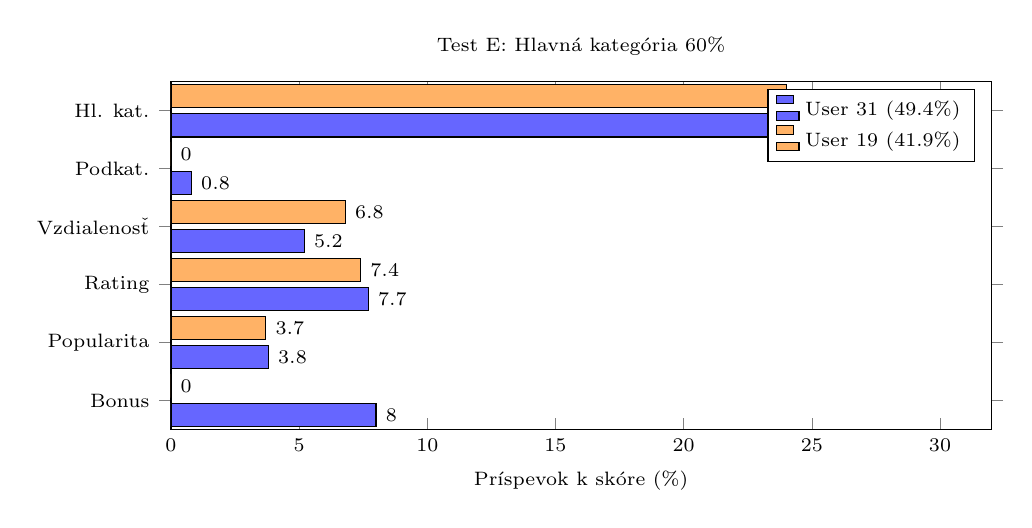
\begin{tikzpicture}
\begin{axis}[
    xbar, width=12cm, height=6cm,
    xlabel={Príspevok k skóre (\%)},
    symbolic y coords={Bonus, Popularita, Rating, Vzdialenosť, Podkat., Hl. kat.},
    ytick=data,
    nodes near coords,
    nodes near coords align={horizontal},
    title={Test E: Hlavná kategória 60\%},
    xmin=0, xmax=32,
    bar width=0.3cm,
]
\addplot[fill=blue!60] coordinates {
    (24.0,Hl. kat.) (0.8,Podkat.) (5.2,Vzdialenosť) (7.7,Rating) (3.8,Popularita) (8.0,Bonus)
};
\addplot[fill=orange!60] coordinates {
    (24.0,Hl. kat.) (0.0,Podkat.) (6.8,Vzdialenosť) (7.4,Rating) (3.7,Popularita) (0.0,Bonus)
};
\legend{User 31 (49.4\%), User 19 (41.9\%)}
\end{axis}
\end{tikzpicture}
\caption{Porovnanie príspevkov faktorov – Test E}
\label{fig:graf_testE}
\end{figure}

Tento test ilustruje silnú personalizáciu podľa histórie: obaja dostali odporúčania z dominantnej kategórie svojej histórie (Music \& Entertainment pre User 31, Sports pre User 19). Pozoruhodné je nižšie celkové skóre v porovnaní s inými testami – kategorizácia má prirodzene nižšie normalizované hodnoty ako rating či obľúbenosť, čo pri jej dominancii znižuje absolútne skóre TOP~1 výsledku.

% ───────────────────────────────────────────────────────────────────────────────
\subsubsection{Test F: Dominancia podkategórie ($w_2 = 60\,\%$)}
% ───────────────────────────────────────────────────────────────────────────────

\begin{table}[H]
\centering
\caption{Konfigurácia váh – Test F}
\label{tab:vahy_testF}
\begin{tabular}{|l|c|}
\hline
\textbf{Faktor} & \textbf{Váha ($w_i$)} \\ \hline
Hlavná kategória ($w_1$) & 8\% \\
Podkategória ($w_2$)     & 60\% \\
Vzdialenosť ($w_3$)      & 8\% \\
Rating ($w_4$)           & 8\% \\
Popularita ($w_5$)       & 8\% \\
Obľúbený bonus ($w_6$)   & 8\% \\ \hline
\textbf{Súčet}           & \textbf{100\%} \\ \hline
\end{tabular}
\end{table}

\begin{table}[H]
\centering
\caption{TOP 1 odporúčanie – Test F}
\label{tab:vysledky_testF}
\small
\begin{tabular}{|l|l|l|}
\hline
 & \textbf{Test User 31} & \textbf{Test User 19} \\ \hline
\textbf{Udalosť}      & udalost 1 \#180         & udalost 10 \#99 \\
\textbf{Kategória}    & Music \& Ent. / DJ Set  & Community \& Social / Street meetup \\
\textbf{Vzdialenosť}  & 13.70 km                & 8.63 km \\
\textbf{Rating}       & 4.6 / 5 (10 hod.)       & 4.1 / 5 (12 hod.) \\
\textbf{Účastníci}    & 7/55                    & 6/30 \\ \hline
\textbf{Celkové skóre} & \textbf{35.0\%}        & \textbf{34.1\%} \\ \hline
Hl. kategória         & 3.2\%                   & 1.6\% \\
Podkategória          & 12.0\%                  & 12.0\% \\
Vzdialenosť           & 3.4\%                   & 4.3\% \\
Rating                & 7.4\%                   & 6.6\% \\
Popularita            & 1.0\%                   & 1.6\% \\
Obľúbený bonus        & 8.0\%                   & 8.0\% \\ \hline
\end{tabular}
\end{table}

\begin{figure}[H]
\centering
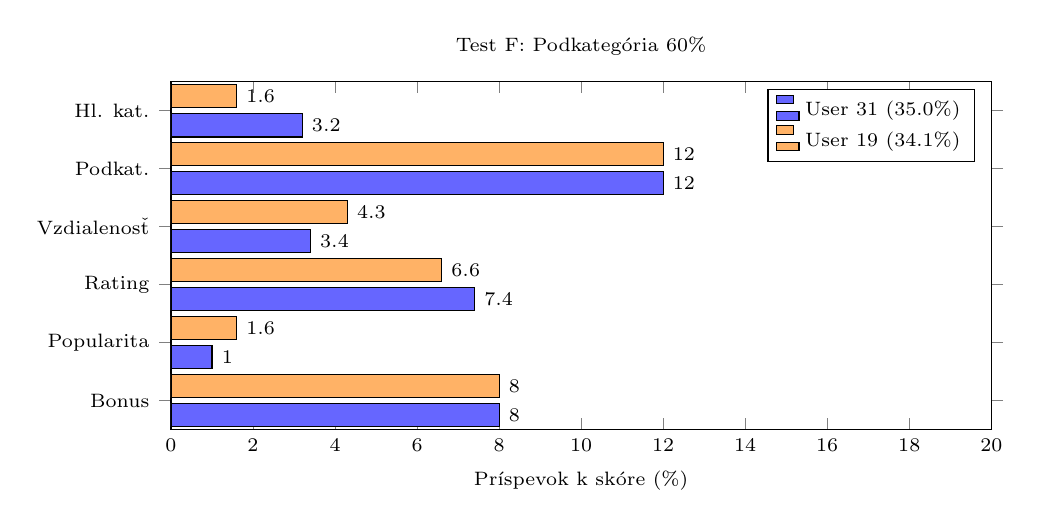
\begin{tikzpicture}
\begin{axis}[
    xbar, width=12cm, height=6cm,
    xlabel={Príspevok k skóre (\%)},
    symbolic y coords={Bonus, Popularita, Rating, Vzdialenosť, Podkat., Hl. kat.},
    ytick=data,
    nodes near coords,
    nodes near coords align={horizontal},
    title={Test F: Podkategória 60\%},
    xmin=0, xmax=20,
    bar width=0.3cm,
]
\addplot[fill=blue!60] coordinates {
    (3.2,Hl. kat.) (12.0,Podkat.) (3.4,Vzdialenosť) (7.4,Rating) (1.0,Popularita) (8.0,Bonus)
};
\addplot[fill=orange!60] coordinates {
    (1.6,Hl. kat.) (12.0,Podkat.) (4.3,Vzdialenosť) (6.6,Rating) (1.6,Popularita) (8.0,Bonus)
};
\legend{User 31 (35.0\%), User 19 (34.1\%)}
\end{axis}
\end{tikzpicture}
\caption{Porovnanie príspevkov faktorov – Test F}
\label{fig:graf_testF}
\end{figure}

Test F produkuje najnižšie absolútne skóre spomedzi všetkých scenárov (35.0\,\% a 34.1\,\%). Podkategória ako faktor s najnižším rozptylom (používateľ navštevuje mnoho rôznych podkategórií) generuje malé normalizované hodnoty, a to aj pri váhe 60\,\%. Napriek tomu systém správne identifikoval podkategórie konzistentné s históriou oboch používateľov – DJ Set pre User 31 (2 návštevy) a Street meetup pre User 19 (1 návšteva + obľúbená).